\documentclass{article}

% if you need to pass options to natbib, use, e.g.:
%     \PassOptionsToPackage{numbers, compress}{natbib}
% before loading neurips_2020

% ready for submission
% \usepackage{neurips_2020}

% to compile a preprint version, e.g., for submission to arXiv, add add the
% [preprint] option:
\usepackage[preprint]{neurips_2020}

% to compile a camera-ready version, add the [final] option, e.g.:
%     \usepackage[final]{neurips_2020}

% to avoid loading the natbib package, add option nonatbib:
%    \usepackage[nonatbib]{neurips_2020}

\usepackage[utf8]{inputenc} % allow utf-8 input
\usepackage[T1]{fontenc}    % use 8-bit T1 fonts
\usepackage{hyperref}       % hyperlinks
\usepackage{url}            % simple URL typesetting
\usepackage{booktabs}       % professional-quality tables
\usepackage{amsfonts}       % blackboard math symbols
\usepackage{nicefrac}       % compact symbols for 1/2, etc.
\usepackage{microtype}      % microtypography
\usepackage{graphicx}
\usepackage{float}
\restylefloat{table}
\usepackage{array}
\usepackage{booktabs, multirow} % for borders and merged ranges
\usepackage{soul}% for underlines
\usepackage[table]{xcolor} % for cell colors
\usepackage{changepage,threeparttable} % for wide tables
\newcolumntype{L}{>{\centering\arraybackslash}m{3cm}}

\title{Formatting Instructions For NeurIPS 2020}

% The \author macro works with any number of authors. There are two commands
% used to separate the names and addresses of multiple authors: \And and \AND.
%
% Using \And between authors leaves it to LaTeX to determine where to break the
% lines. Using \AND forces a line break at that point. So, if LaTeX puts 3 of 4
% authors names on the first line, and the last on the second line, try using
% \AND instead of \And before the third author name.

\title{Understanding gender violence depiction in online news media}

\author{Caitlin Loftus \\
	\texttt{cloftus@uchicago.edu}  \\
	The University of Chicago
	\AND
	Roberto Barroso-Luque\\
	\texttt{barrosoluquer@uchicago.edu} \\
    The University of Chicago\\
	\AND
	Rukhshan Mian\\
	\texttt{rukhshan@uchicago.edu} \\
	The University of Chicago\\}

\begin{document}
\maketitle

\begin{abstract}{
		Our study blabla
	}
\end{abstract}

\newpage
\section{Introduction and Background}{
BLABLABLA

}
\newpage

\section{Methodology}{
	
\subsection{Web Scrapping}{
%Please add the following packages if necessary:
%\usepackage{booktabs, multirow} % for borders and merged ranges
%\usepackage{soul}% for underlines
%\usepackage[table]{xcolor} % for cell colors
%\usepackage{changepage,threeparttable} % for wide tables
%If the table is too wide, replace \begin{table}[!htp]...\end{table} with
%\begin{adjustwidth}{-2.5 cm}{-2.5 cm}\centering\begin{threeparttable}[!htb]...\end{threeparttable}\end{adjustwidth}
\begin{table}[!htp]\centering
	\caption{Article and Newspaper Counts}\label{tab: }
	\scriptsize
	\begin{tabular}{lrrrr}\toprule
		&\textbf{Newspaper} &\textbf{Political ideology} &\textbf{Number of articles} \\\midrule
		\multirow{3}{*}{Mexico} &El Heraldo &Right &2820 \\
		&El Universal &Centre &3513 \\
		&La Jornada &Left &2099 \\
		& & & \\
		\multirow{3}{*}{Pakistan} &Nation &Centre-Right &968 \\
		&Dawn &Centre-Left &330 \\
		&The News &Centre-Left &930 \\
		& & & \\
		\multirow{3}{*}{UK} &The Times &Centre-right &1206 \\
		&The Sun &Right &1269 \\
		&The Guardian &Left &4568 \\
		& & & \\
		Total & & &17778 \\
		\bottomrule
	\end{tabular}
\end{table}

}



	
	
}
\newpage


\section{Results}{	
\subsection{Word Embedings (Word2Vec)}{

\begin{figure}[H]
	\center{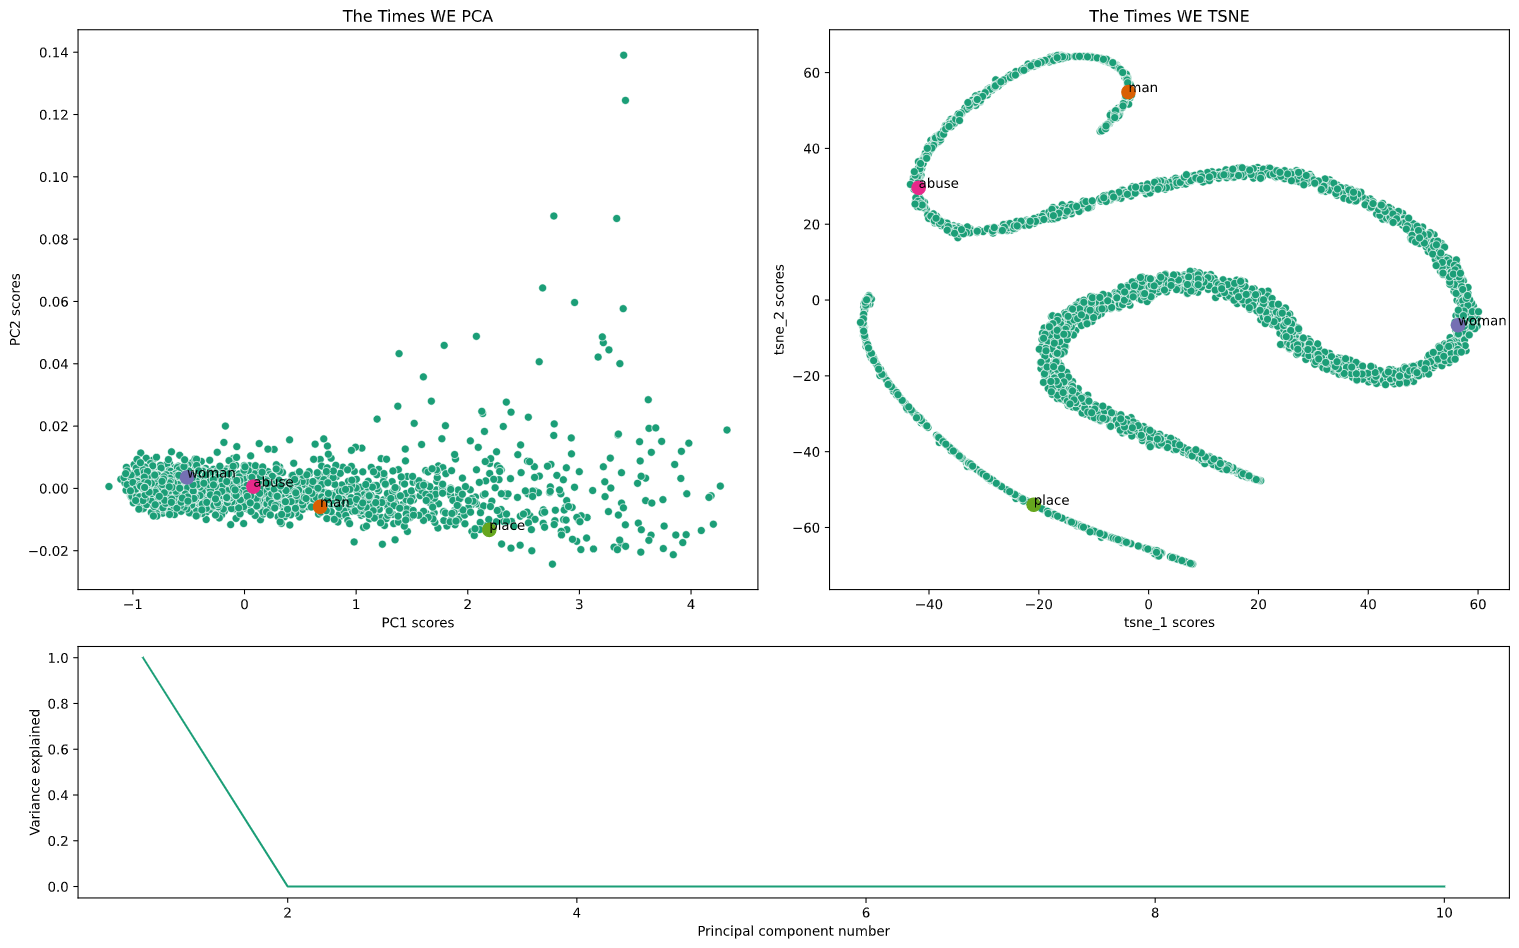
\includegraphics[width=\textwidth]
		{figures/thetimeswe.png}}
	\caption{\label{fig:my-label1} Visualization of embedding space (The Times UK)}
\end{figure}

\begin{figure}[H]
	\center{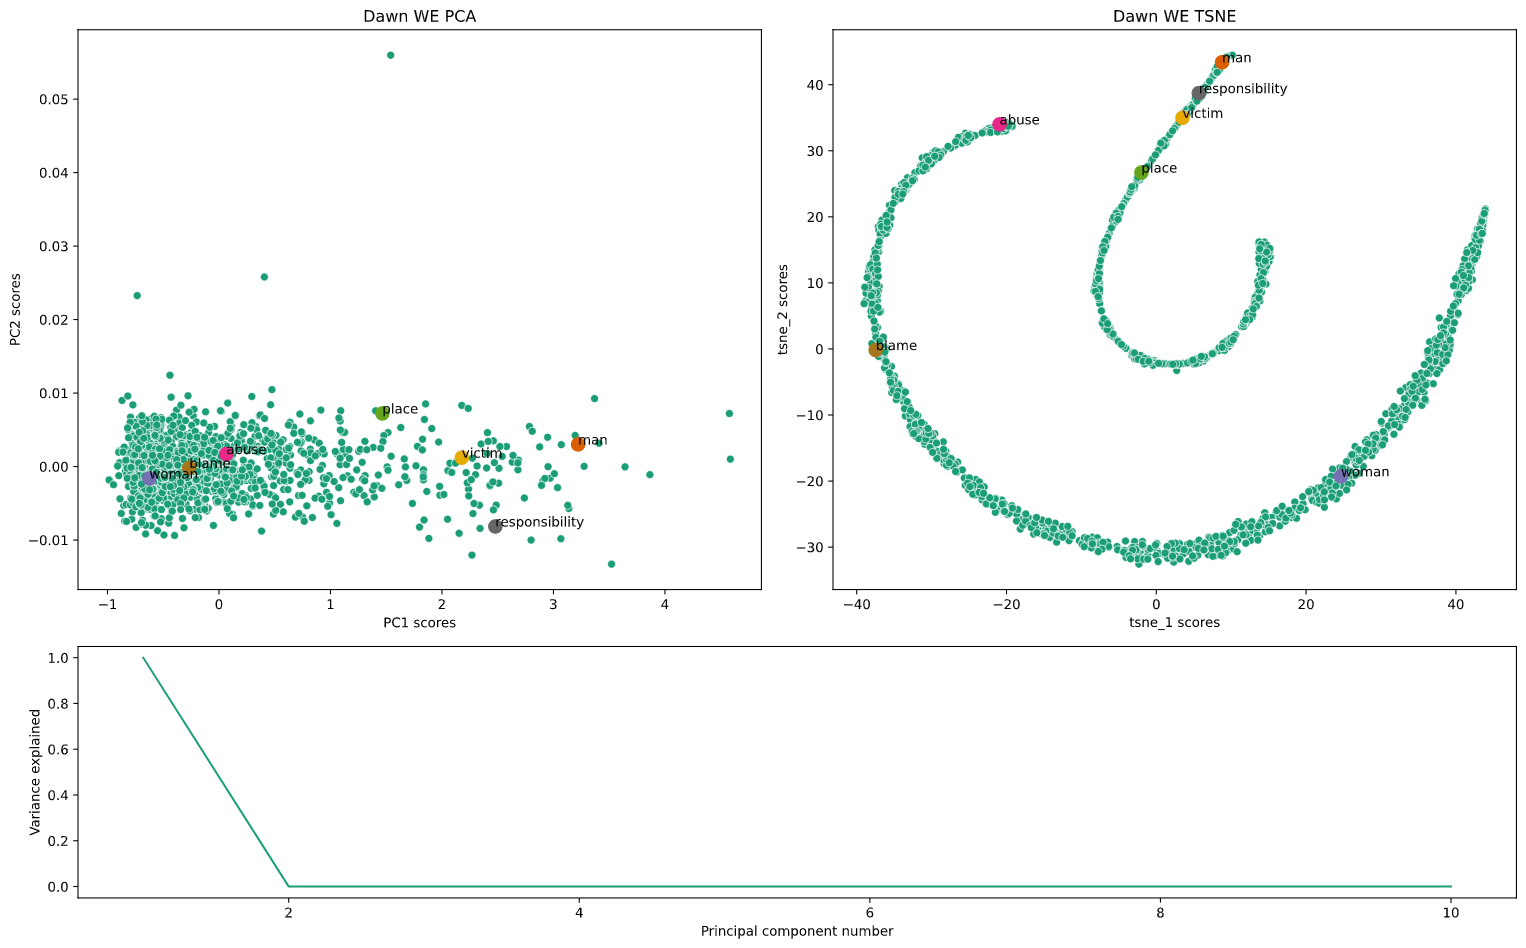
\includegraphics[width=\textwidth]
		{figures/dawnwe.png}}
	\caption{\label{fig:my-label1} Visualization of embedding space (Dawn Pakistan)}
\end{figure}

\begin{figure}[H]
	\center{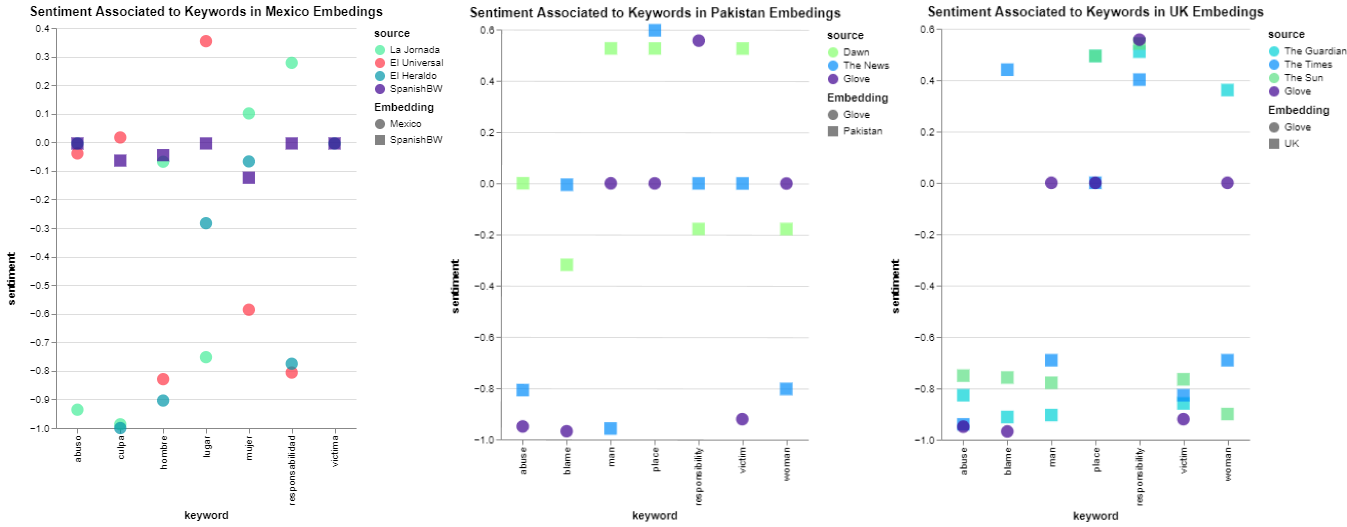
\includegraphics[width=\textwidth]
		{figures/sentimentfig.png}}
	\caption{\label{fig:my-label1} Sentiment towards keywords}
\end{figure}

\begin{equation} \label{eu_eqn}
	 analogy(m:w \rightarrow k:?) = argmax_{v,w,k}(cos(v,k)-cos(v,m)+cos(v,w)))
\end{equation}


%Please add the following packages if necessary:
%If the table is too wide, replace \begin{table}[!htp]...\end{table} with
\begin{table}[!htp]\centering
	\caption{Semantic Algebra: $w_{woman}+ w_{victim} - w_{man} = ??$}\label{tab: }
	\scriptsize
	\begin{tabular}{lrrrr}\toprule
		&\textbf{Newspaper} &\textbf{Political ideology} &\textbf{Result} \\\midrule
		\multirow{3}{*}{Mexico} &El Heraldo &Right &('expresión', 0.91), ('condición', 0.90), ('completa', 0.89), ('ideología', 0.88), ('conlleva', 0.88) \\
		&El Universal &Centre &('libre', 0.92), ('política', 0.92), ('manpowergroup', 0.92), ('crueldad', 0.92), ('erradicar', 0.92) \\
		&La Jornada &Left &('definición', 0.82), ('subordinación', 0.82), ('violenta', 0.81), ('mujerla', 0.81), ('castiga', 0.80) \\
		& & &\textbf{} \\
		\multirow{3}{*}{Pakistan} &Nation &Centre-Right & \\
		&Dawn &Centre-Left &('report', 0.99), ('police', 0.99), ('law', 0.99), ('state', 0.99), ('society', 0.9998923540115356) \\
		&The News &Centre-Left &[('domestic', 0.99), ('harassment', 0.99), ('country', 0.99), ('increase', 0.99), ('rise', 0.99) \\
		&\textbf{} &\textbf{} &\textbf{} \\
		\multirow{3}{*}{UK} &The Sun &Right &('survivor', 0.75), ('domestic', 0.75), ('harassment', 0.73), ('demand', 0.71), ('mutilation', 0.71) \\
		&The Times &Centre-right &('charge', 0.99), ('offence', 0.99), ('allege', 0.99), ('violence', 0.99), ('report', 0.99) \\
		&The Guardian &Left &('survivor', 0.71), ('perpetrator', 0.53), ('domestic', 0.49), ('abuser', 0.48), , ('stalker', 0.44) \\
		\bottomrule
	\end{tabular}
\end{table}

}
	
}
\newpage
\section{Conclusion, further research and limitations}{
BLABLABLA
}


\section{Appendix}{

\begin{figure}[H]
	\center{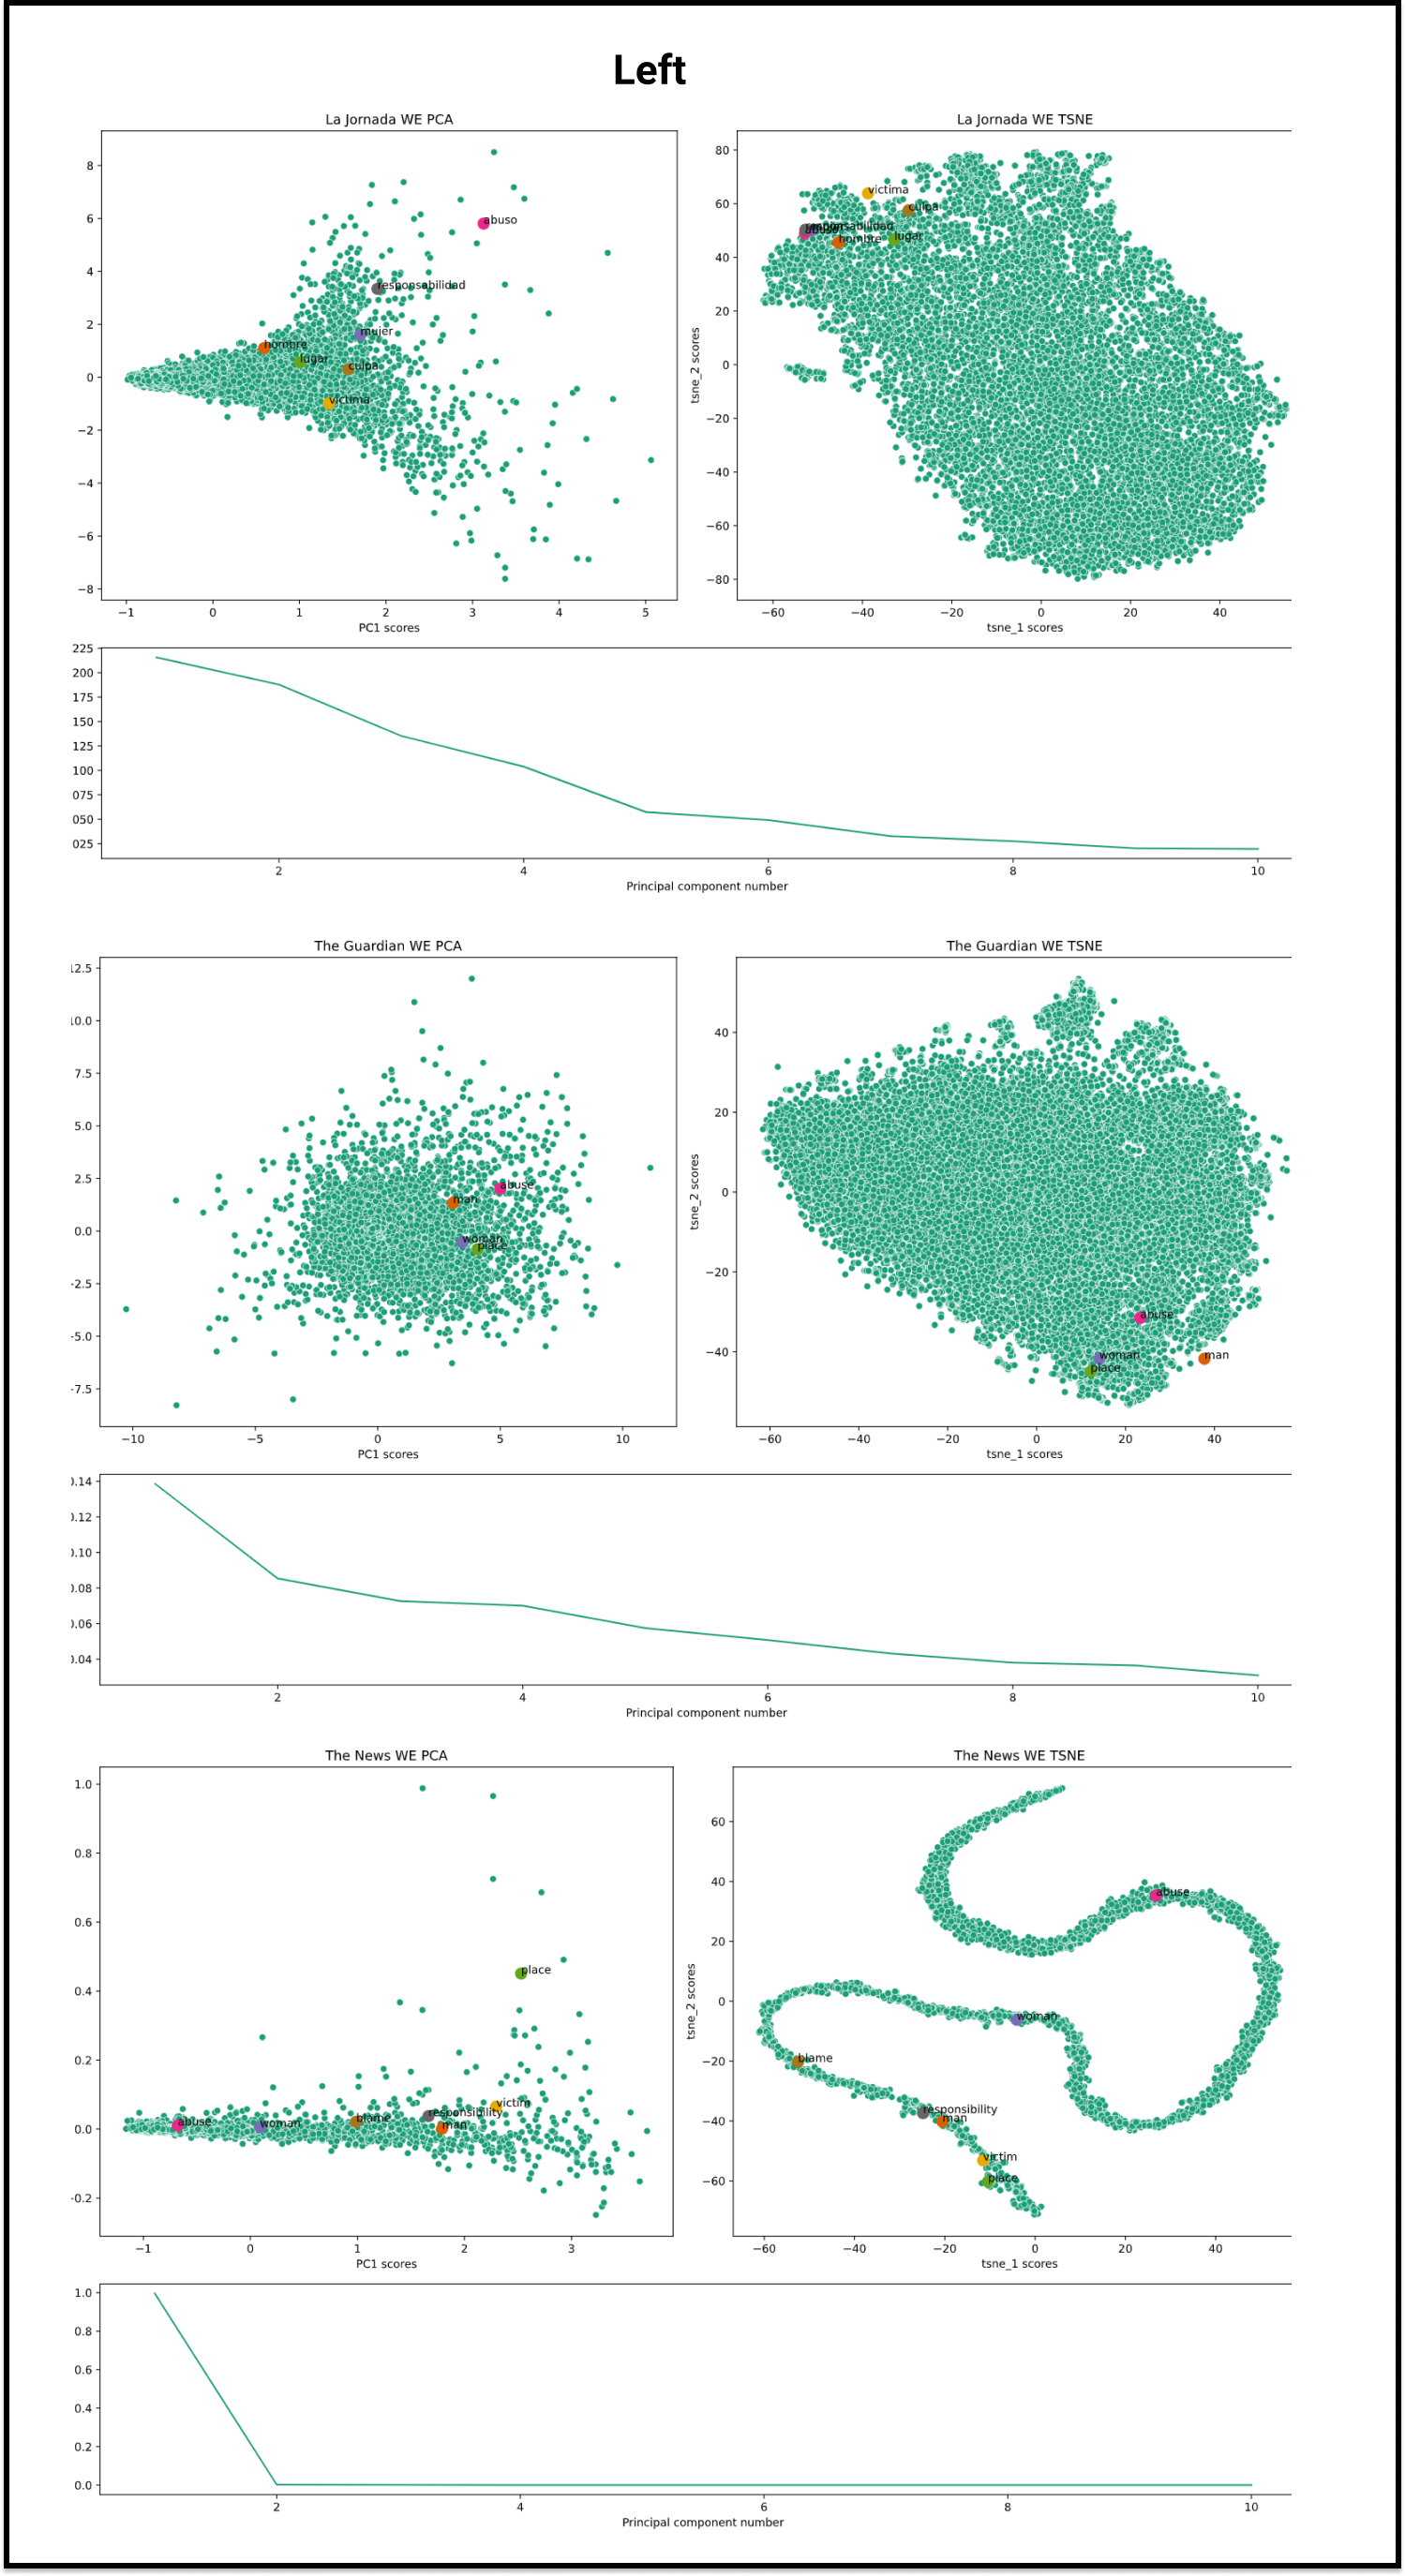
\includegraphics[width=\textwidth,height=\textheight,keepaspectratio]
		{figures/leftwe.png}}
	\caption{\label{fig:my-label1} GBV depiction in left leaning media}
\end{figure}


\begin{figure}[H]
	\center{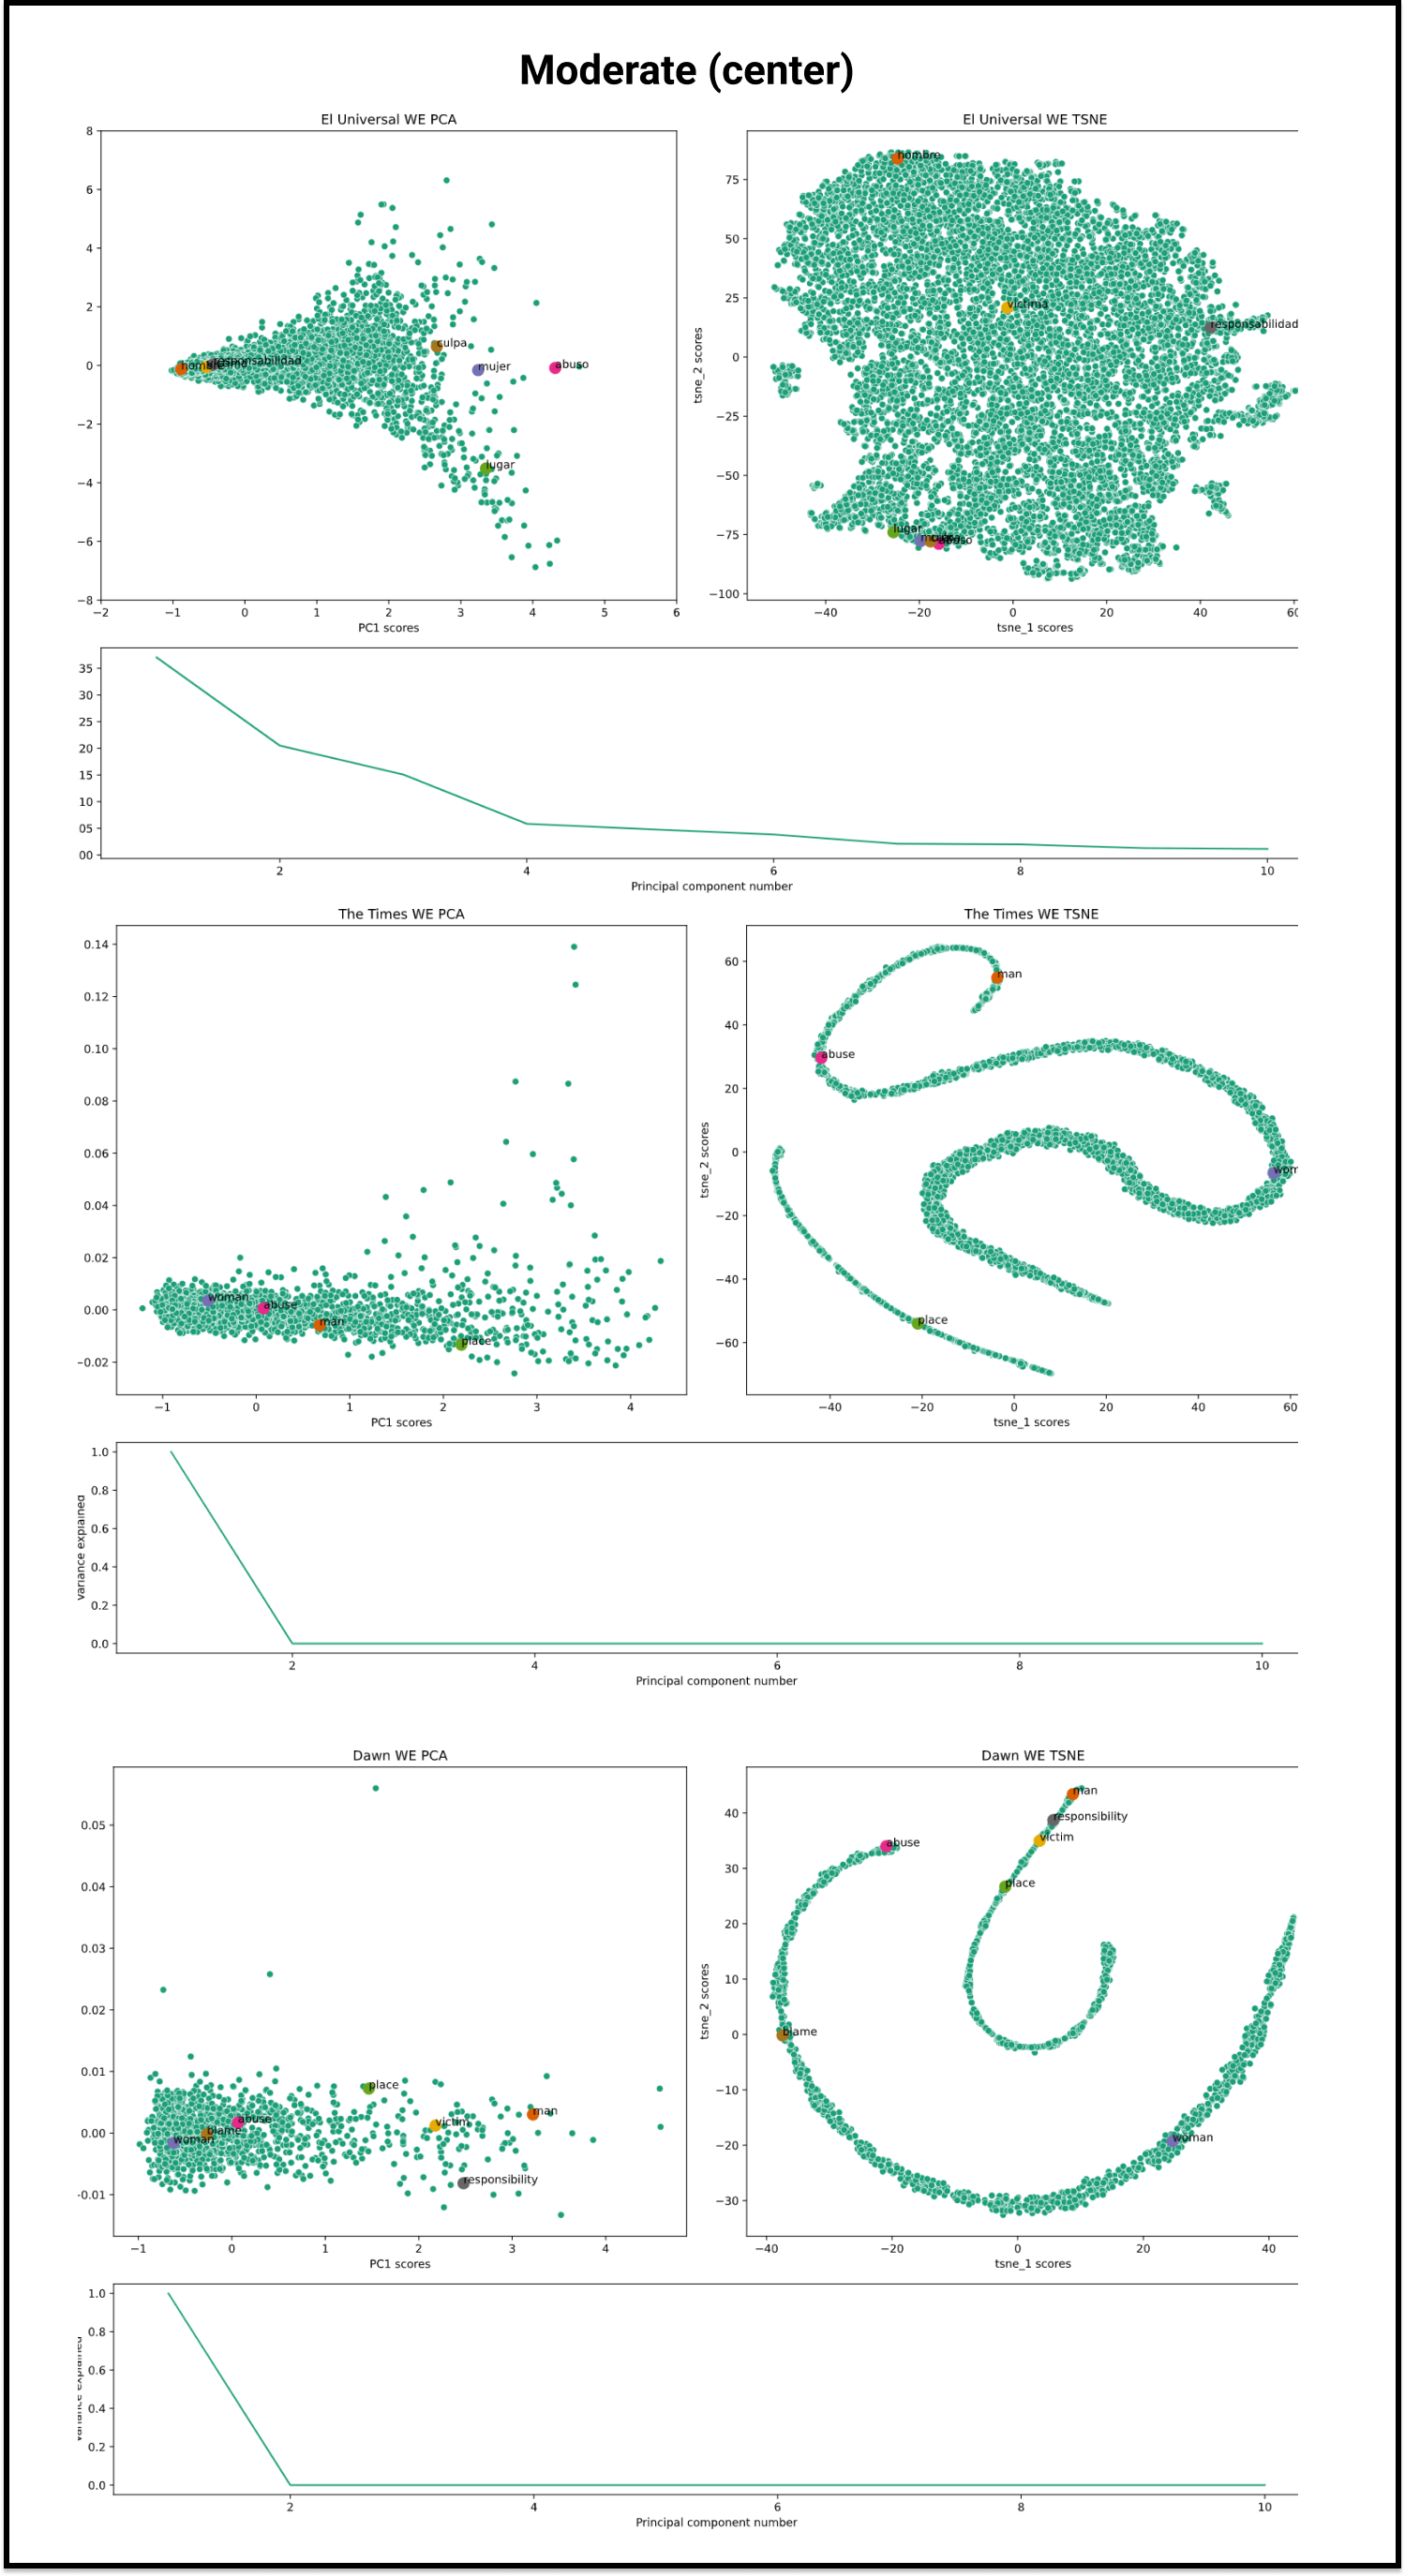
\includegraphics[width=\textwidth,height=\textheight,keepaspectratio]
		{figures/centerwe.png}}
	\caption{\label{fig:my-label1} GBV depiction in moderate media}
\end{figure}

\begin{figure}[H]
	\center{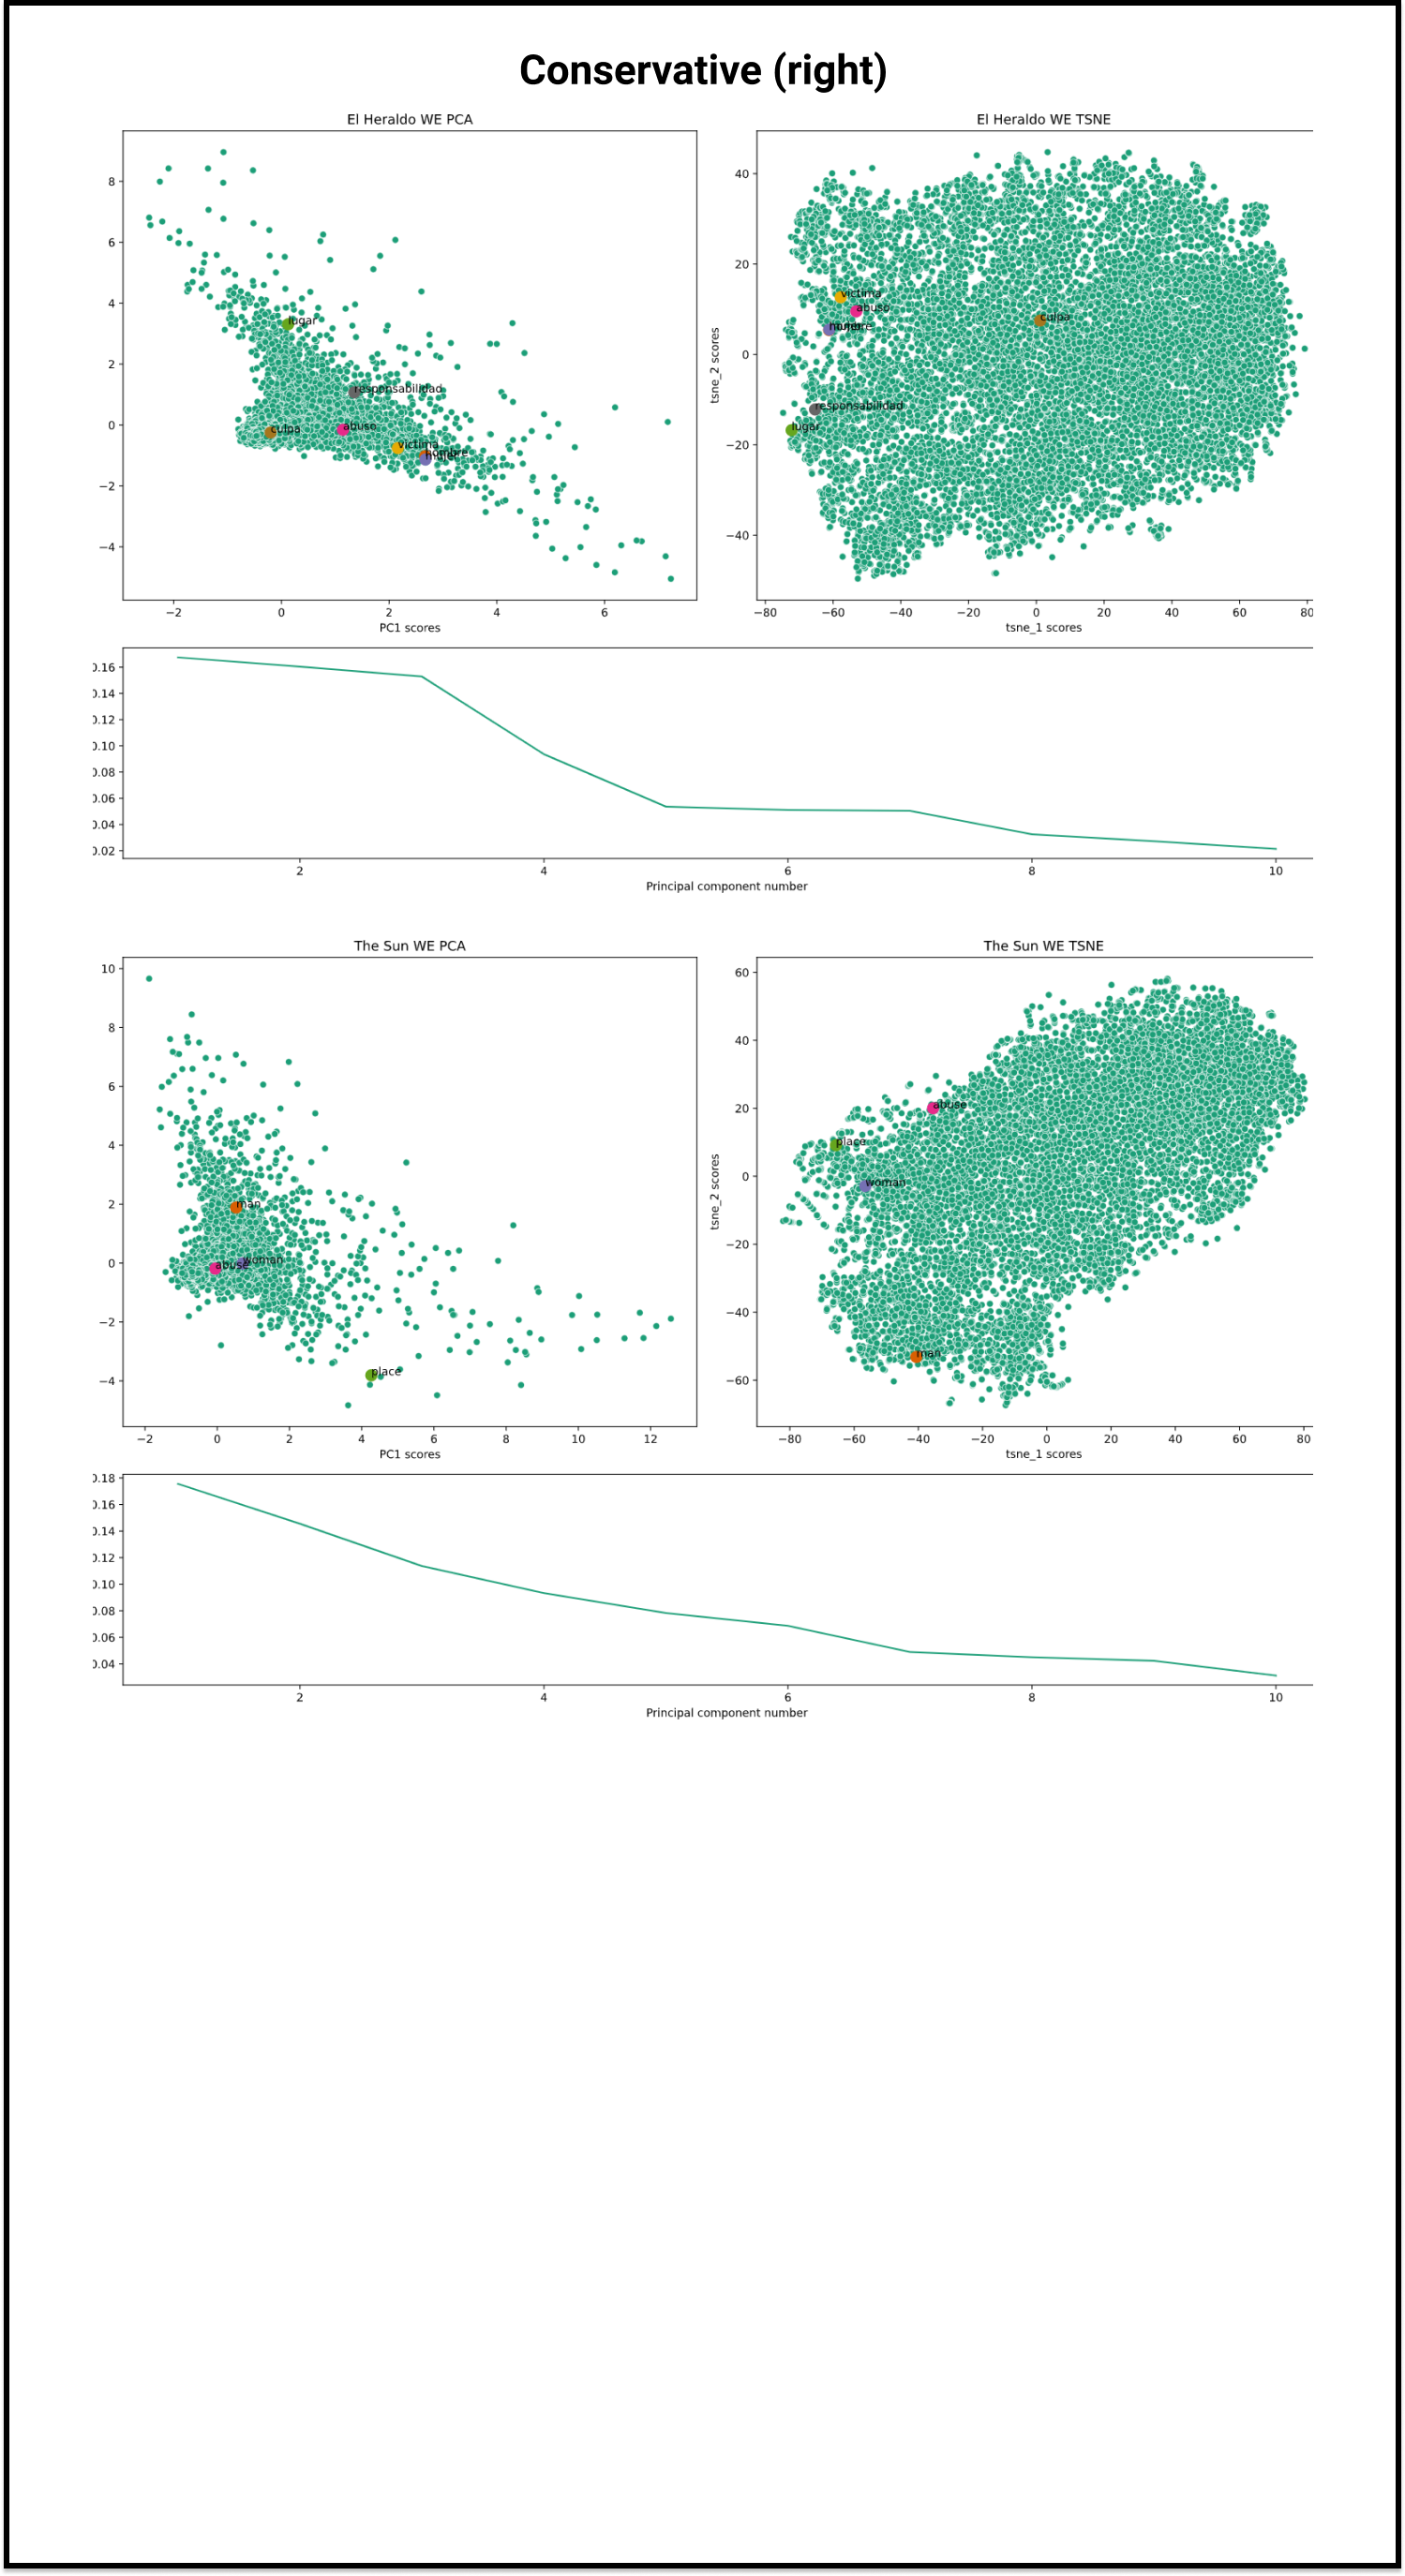
\includegraphics[width=\textwidth,height=\textheight,keepaspectratio]
		{figures/rightwe.png}}
	\caption{\label{fig:my-label1} GBV depiction right leaning media}
\end{figure}

}




\section{References}\label{sec_ref}

[1] Bello, H. J., Palomar, N., Gallego, E., Navascués, L. J., and Lozano, C. (2020). Machine Learning to study the impact of gender-based violence in the news media. arXiv preprint arXiv:2012.07490.

[2] Busso, L., Combei, C. R., amd Tordini, O. (2020). Narrating Gender Violence A Corpus-Based Study on the Representation of Gender-Based Violence in Italian Media. In G. Giusti, and G. Iannàccaro (Eds.), Language, Gender and Hate Speech : A Multidisciplinary Approach (Language, Gender and Hate Speech A Multidisciplinary Approach). https://doi.org/10.30687/978-88-6969-478-3/002

[3] , A., Bryson, J. J., and Narayanan, A. (2017). Semantics derived automatically from language corpora contain human-like biases. Science, 356(6334), 183-186. doi:10.1126/science.aal4230

[4]Bail, C. A. (2012). The fringe effect. American Sociological Review, 77(6), 855-879. doi:10.1177/0003122412465743

[5]Kozlowski, A. C., Taddy, M., and Evans, J. A. (2019). The geometry of culture: Analyzing the meanings of class through word embeddings. American Sociological Review, 84(5), 905-949. doi:10.1177/0003122419877135

[6]Sendén, M. G., Sikström, S., and Lindholm, T. (2015). “She” and “He” in news media messages: Pronoun use reflects gender biases in semantic contexts. Sex Roles, 72(1-2), 40-49. doi: 10.1007/s11199-014-0437-x

[7]Von Nordheim, G., Muller, H., and Scheppe, M. (2019). Young, free and biased: A comparison of mainstream and right-wing media coverage of the 2015–16 refugee crisis in German newspapers. Journal of Alternative and Community Media, 4(1), 38-56. doi:10.1386/joacm000421
 
[8]Grimmer J. \& Stewart B.M (2013): Text as Data: The Promise and Pitfalls of Automatic Content Analysis Methods for Political Texts. 
{\it Political Analysis}

\newpage
\pagebreak




\end{document}
